% Figure 3 uses the native TikZ artwork below.
% Required packages:
% \usepackage{tikz}
% \usetikzlibrary{arrows.meta,positioning,fit,backgrounds,shapes.geometric,calc}
% \usepackage{xcolor}
% \usepackage{graphicx}

\begin{figure*}[t]
\centering
\resizebox{0.68\textwidth}{!}{%
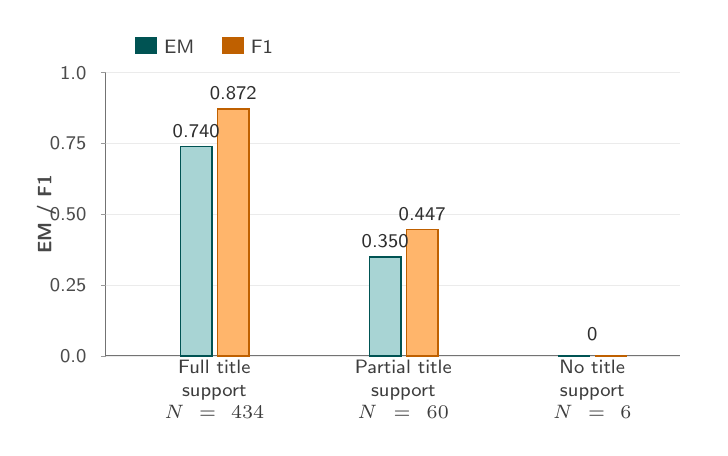
\begin{tikzpicture}[
    font=\sffamily\footnotesize,
    axis/.style={draw=black!55, line width=0.55pt},
    tick/.style={draw=black!40, line width=0.45pt},
    grid/.style={draw=black!8, line width=0.35pt},
    axislabel/.style={font=\sffamily\bfseries\scriptsize, text=black!72},
    barlabel/.style={font=\sffamily\scriptsize, align=center, text=black!76},
    value/.style={font=\sffamily\scriptsize, text=black!82},
    legend/.style={font=\sffamily\scriptsize, align=left, text=black!76}
]

% Supporting-title buckets and answer quality.
\begin{scope}[shift={(0,0)}]
    \draw[axis] (0,0) -- (7.3,0);
    \draw[axis] (0,0) -- (0,3.6);
    \foreach \y/\lab in {0/0.0,0.9/0.25,1.8/0.50,2.7/0.75,3.6/1.0} {
        \draw[tick] (-0.06,\y) -- (0,\y);
        \node[anchor=east, font=\sffamily\scriptsize, text=black!70] at (-0.12,\y) {\lab};
        \draw[grid] (0,\y) -- (7.3,\y);
    }
    \node[rotate=90, axislabel] at (-0.75,1.8) {EM / F1};

    % HyDE full title support: EM=.7396, F1=.8720
    \fill[teal!34] (0.95,0) rectangle (1.35,2.663);
    \draw[teal!65!black, line width=0.55pt] (0.95,0) rectangle (1.35,2.663);
    \fill[orange!58] (1.42,0) rectangle (1.82,3.139);
    \draw[orange!75!black, line width=0.55pt] (1.42,0) rectangle (1.82,3.139);
    \node[value] at (1.15,2.86) {0.740};
    \node[value] at (1.62,3.34) {0.872};
    \node[barlabel, text width=27mm] at (1.38,-0.42) {Full title\\support\\$N=434$};

    % HyDE partial title support: EM=.3500, F1=.4472
    \fill[teal!34] (3.35,0) rectangle (3.75,1.260);
    \draw[teal!65!black, line width=0.55pt] (3.35,0) rectangle (3.75,1.260);
    \fill[orange!58] (3.82,0) rectangle (4.22,1.610);
    \draw[orange!75!black, line width=0.55pt] (3.82,0) rectangle (4.22,1.610);
    \node[value] at (3.55,1.46) {0.350};
    \node[value] at (4.02,1.81) {0.447};
    \node[barlabel, text width=28mm] at (3.78,-0.42) {Partial title\\support\\$N=60$};

    % HyDE no title support: both metrics are zero; the small bucket is labeled without extra decimals.
    \draw[teal!65!black, line width=0.55pt] (5.75,0) -- (6.15,0);
    \draw[orange!75!black, line width=0.55pt] (6.22,0) -- (6.62,0);
    \node[value] at (6.18,0.28) {0};
    \node[barlabel, text width=25mm] at (6.18,-0.42) {No title\\support\\$N=6$};

    \node[legend, anchor=west] at (0.25,3.95) {\textcolor{teal!65!black}{\rule{8pt}{6pt}} EM \quad \textcolor{orange!75!black}{\rule{8pt}{6pt}} F1};
\end{scope}

\end{tikzpicture}%
}
\caption{Supporting-title completeness and answer quality on HotpotQA. The figure groups HyDE-style RAG examples by retrieved supporting-title completeness and reports EM/F1 within each bucket. Full title support means that all annotated supporting titles are retrieved in the top-10 evidence set. The no-title-support bucket contains only six examples and is reported descriptively. The single-annotator EM-mismatch taxonomy is reported separately in the supplement as a descriptive diagnostic.}
\label{fig:evidence_error_taxonomy}
\end{figure*}
